% !TEX = root../thesis.tex

\chapter{Experimental Apparatus}
\label{chap:exp}

\section{The Large Hadron Collider} \label{sec:LHC}
% Overview
The Large Hadron Collider (LHC) is a circular collider spanning the border between France and Switzerland, based at the European Organization for Nuclear Research (CERN). The central features of the LHC are the superconducting rings, located about 100 m underground with a circumference of 27 km, designed to collide counter-rotating beams of protons or heavy ions at highly relativistic energies. Along the rings lie four major experiments: ATLAS, CMS, ALICE, and LHCb. Both ALTAS and CMS are general purpose detectors, designed to probe a wide range of physics including the Higgs boson, precision measurements of fundamental constants, and physics beyond the standard model (BSM). The remaining two experiments are more specialized; ALICE measures quark gluon plasma produced in heavy ion collisions and LHCb focuses on $b$-quark physics and CP violation.

% Lumi and CoM energy
Two prominent aspects of the LHC are the high center of mass energy, referred to using the Mandelstam variable $\sqrt{s}$, and high instantaneous luminosity $\lumi$, often referred to as just luminosity. High $\sqrt{s}$ allows for the production of more massive particles, giving more access to possible BSM physics, while high luminosity is essential for measuring rare processes and precision measurements. A process with cross section $\sigma$ will have a rate $R$ given by

\begin{equation}
	R=\lumi\sigma
\end{equation}

The cross section $\sigma$ is a measure of how probably a process is to occur, and is in units of area. They are frequently measured in $\unit{barns}$, where $1\unit{b} = 100\unit{fm^2}$. Conversely, luminosity uses units of $\unit{Hz/b}$. In cases where the relevant quantity is the total number of events, the integrated luminosity can be defined as $\intlumi=\int{\lumi\dd{t}}$ to give
\begin{equation}
	N_\mathrm{events} = \intlumi\sigma
\end{equation}

The luminosity depends on the characteristics of the proton beam and can be written in terms of the operational parameters of the detector given by

\begin{equation}
	\lumi=\frac{N_b^2n_bf_\mathrm{rev}\gamma_r}{4\pi\epsilon_n\beta^*}F
\end{equation}

where $N_b$ is the number of particles per bunch, $n_b$ is the number of bunches per ring, $f_\mathrm{rev}$ is the LHC revolution frequency, $\gamma_r$ is the Lorentz factor for the proton, $\epsilon_n$ is the transverse normalized beam emittance, $\beta^*$ is the amplitude function at the collision point, and $F$ is a geometric reduction factor based on the crossing angle of the two beams. The nominal design parameters of the LHC were intended to support a peak luminosity of $12\unit{Hz/nb}$~\cite{Bruning:782076}, but during run 2 was able to achieve nearly twice that value at $21.4\unit{Hz/nb}$. The LHC produced $41.6\unit{fb^{-1}}$ in 2016, $49.8\unit{fb^{-1}}$ in 2017, and $67.9\unit{fb^{-1}}$ in 2018 for a total of $159.3\unit{fb^{-1}}$.

\begin{figure}[!htbp]
	\centering
	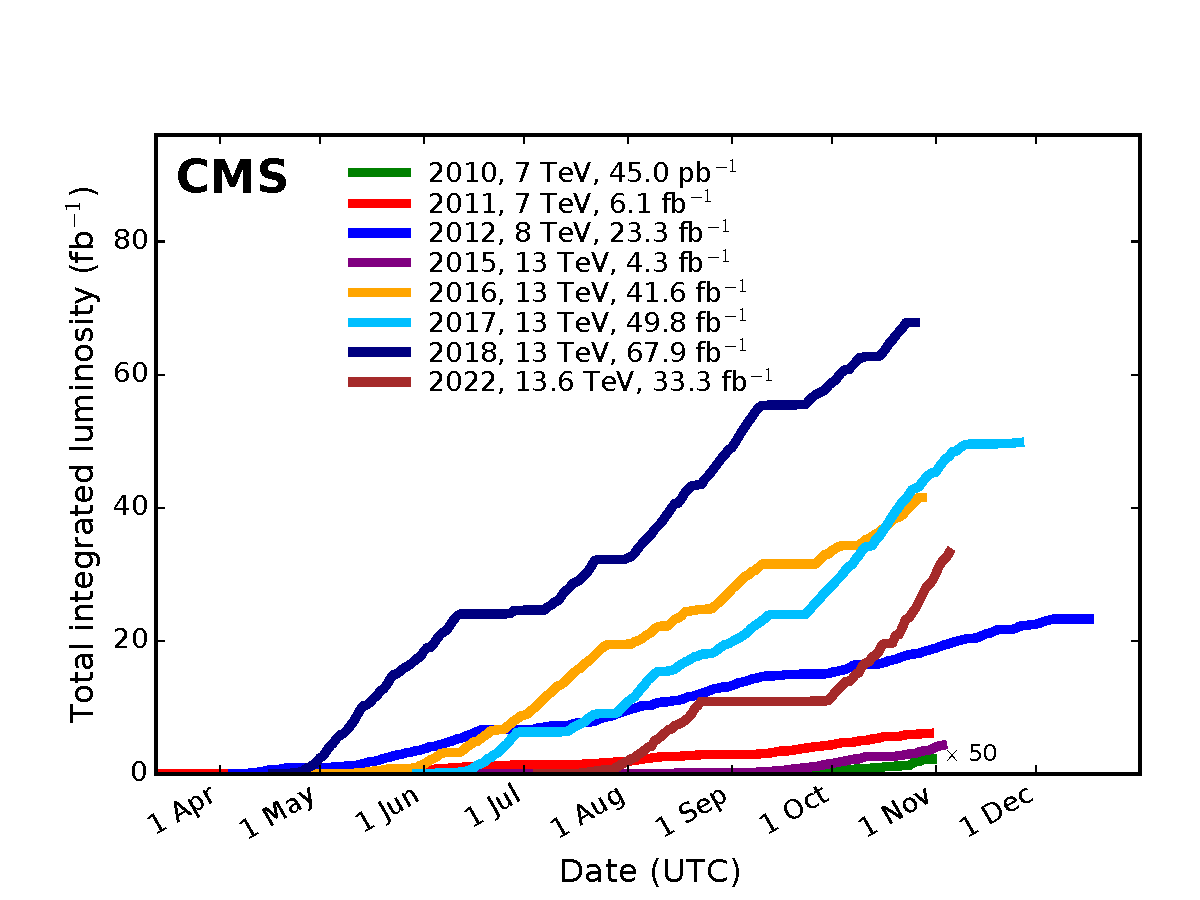
\includegraphics[width=0.34\textwidth]{figs/03_experiment/int_lumi_cumulative_pp_2.pdf}
	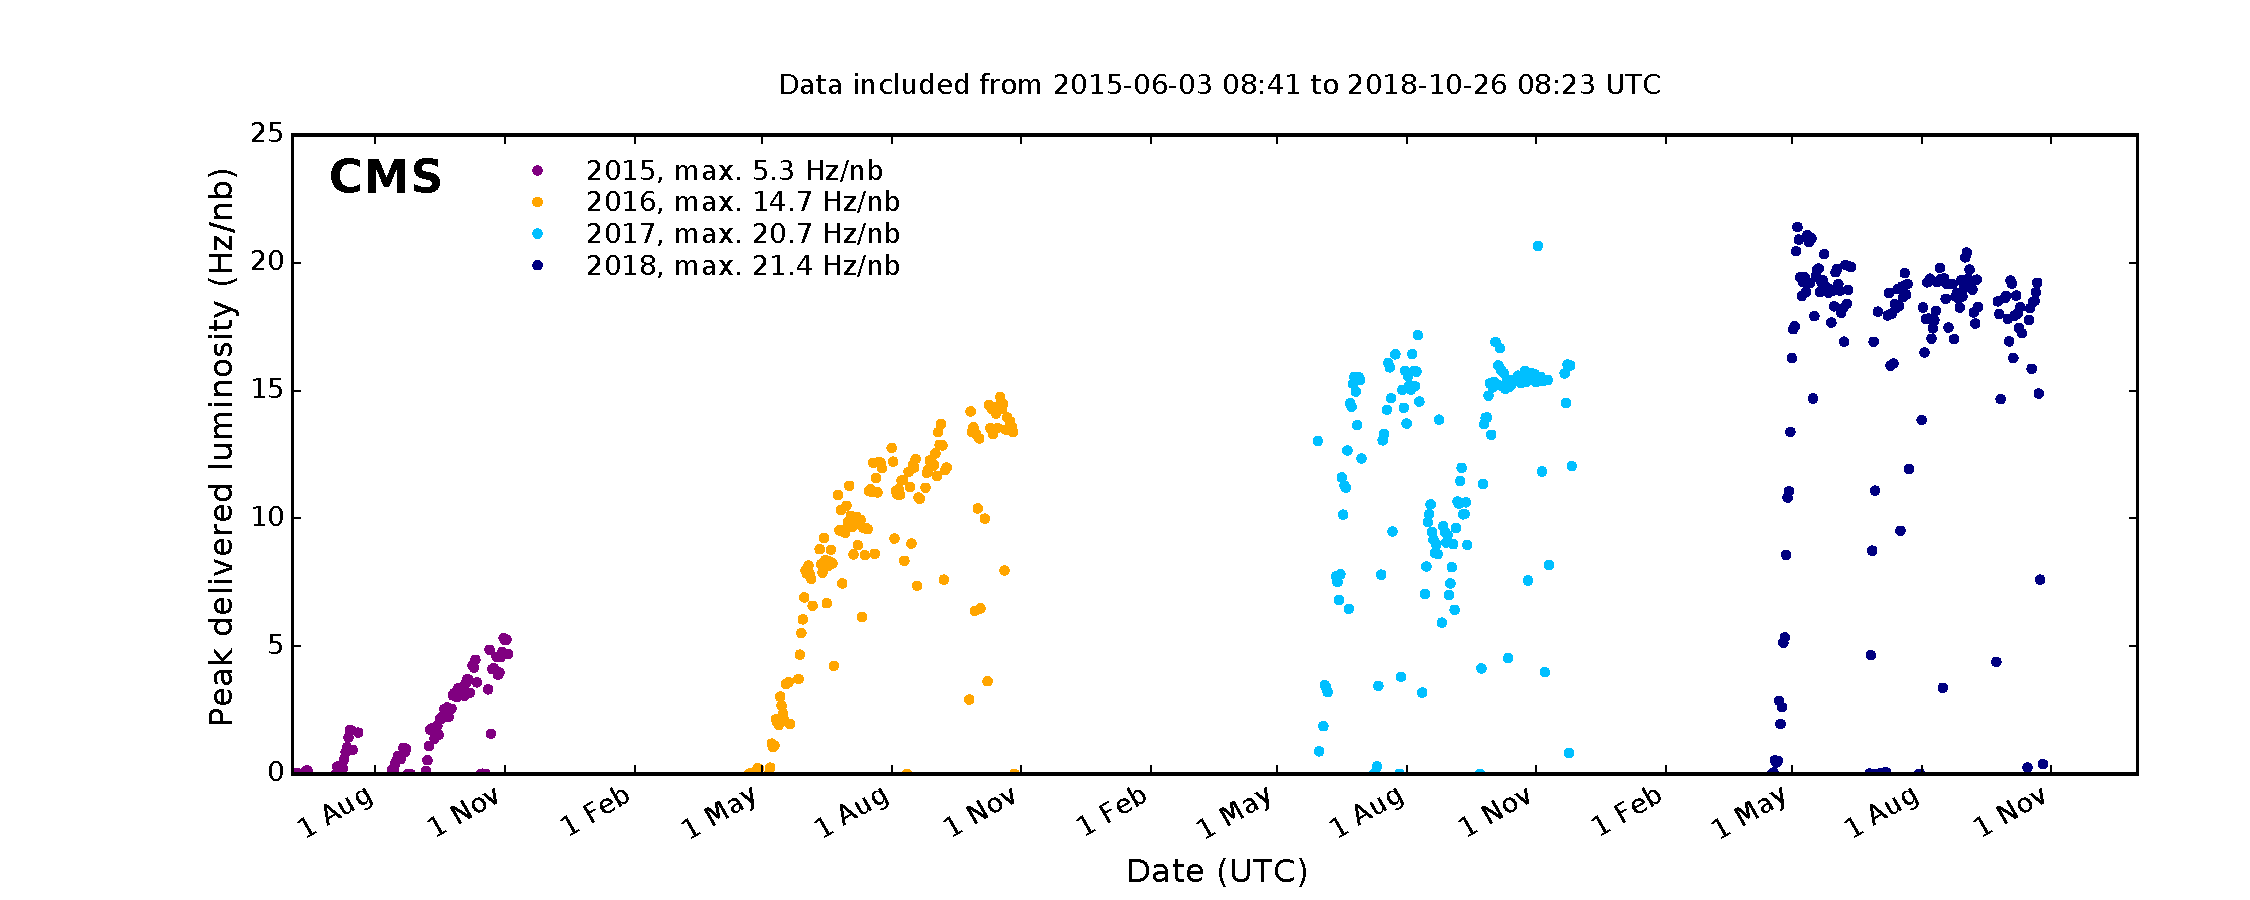
\includegraphics[width=0.65\textwidth]{figs/03_experiment/peak_lumi_pp_run2.pdf}
	\caption[LHC luminosity report. Left: breakdown of the CMS integrated luminosity by year from 2010-2022. Right:  peak luminosity from 2016-2018 data taking~\cite{CMSlumi}.]{LHC luminosity report. Left: breakdown of the CMS integrated luminosity by year from 2010-2022. Right: peak instantaneous luminosity from 2016-2018 data taking~\cite{CMSlumi}}
	\label{fig:LHC_intLumi}
\end{figure}

\begin{comment}
\begin{table}[htb!]
	\caption{Description of beam parameters used to calculate the LHC luminosity, obtained from~\cite{Workman:2022ynf} and~\cite{Herr:941318}}
	\begin{center}
		\begin{tabular}{l l l}
			\hline
			Parameter & Description & Value \\
			\hline
			$N_b$ & Number of particles per bunch & $1.1\times10^{11}$\\
			$n_b$ & Number of bunches per event & $2556$\\
			$f_\mathrm{rev}$ & Revolution frequency & $11.245\unit{kHz}$\\
			$\gamma_r$ & Lorentz factor & $6929.6$\\
			$\epsilon_n$ & Transverse normalized beam emittance & $3.75\unit{\mu m\times rad}$\\
			$\beta^*$ & Amplitude function at collision point & $0.3\unit{m}$\\
			$F$ & Geometric luminosity reduction factor & 0.835\\
			\hline
		\end{tabular}
	\end{center}
\end{table}
\end{comment}

% Proton beams
The protons used in collisions begin as hydrogen atoms, which are first ionized using electric fields to strip the electrons. They are first accelerated to $50\unit{MeV}$ through a linear accelerator Linac2 before entering the Proton Synchrotron Booster (PSB), where they will reach a kinetic energy of $1.4\unit{GeV}$. Next, the protons are accelerated by the Proton Synchrotron (PS) and Super Proton Synchrotron (SPS), where they are accelerated to $26\unit{GeV}$ and $450\unit{GeV}$ respectively. Finally, the beams are injected into the LHC where they undergo acceleration to $6.5\unit{TeV}$, producing the desired center of mass energy of $\sqrt{s}=13\unit{TeV}$.

\begin{figure}[htbp]
	\centering
	\includegraphics[width=0.825\textwidth]{figs/03_experiment/CCC-v2018-print-v2.pdf}
	\caption[Diagram of the CERN accelerator complex during 2018 data taking. Protons begin as hydrogen atoms at Linac2 and collide at various detectors along the LHC at $\sqrt{s}=13\unit{TeV}$]
	{Diagram of the CERN accelerator complex during 2018 data taking~\cite{Mobs:2636343}. Protons begin as hydrogen atoms at Linac2 and are accelerated in several stages to reach $6.5\unit{TeV}$} 
	\label{fig:LHC}
\end{figure}

